\documentclass[12pt]{book} 

\usepackage{amsmath}
\usepackage{graphicx}
\usepackage{import}
\usepackage{amsfonts}
\usepackage{booktabs}

\setlength{\parindent}{0em}  % sets auto indent at new paragraph to none

\newcommand{\incfig}[1]{%
    \import{./figures/}{#1.pdf_tex}
}

\title{\coursetitle\linebreak\lecturename}
\author{\\Cain Susko\\ 
           \\ \\ \\
      Queen's University 
    \\School of Computing\\} 

%=-=-=-=-=-title-=-=-=-=-=%
\newcommand{\lecturename}{Context Free Grammar Pumping Lemma Examples}
\newcommand{\coursetitle}{Software Specifications}
%=-=-=-=-=-#####-=-=-=-=-=%

\begin{document}
\begin{titlepage}
        \maketitle
\end{titlepage}


\section*{Example}

\begin{figure}[h]
        \centering
        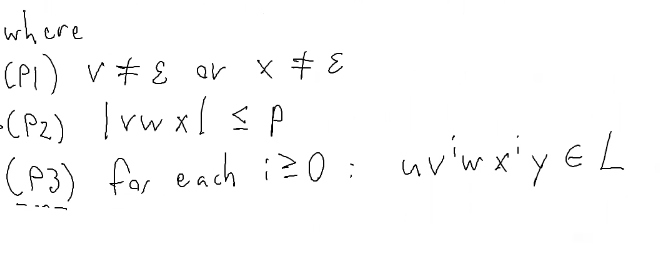
\includegraphics{./figures/pumpingLemma.png}
\end{figure}
Consider the Language of Squares:
\[
L_2 = \{ww \mid w\in\{a,b\}*\}
.\] 
The claim is that $L_2$ is not context free.

Note: showing that $L_2$ is not CF, roughly speaking, shows that variable declarations
cannot be specified with CF Grammars.
\paragraph{attempt 1}
The Question is what string $s$ should we use to derive a contradiction with the 
Pumping Lemma? The first (bad) idea for $s$ is the following:
 \[
s = a^pba^pb\in L_2\\
.\] 
\[
s = a^{p-1}aba^{p-1}b
.\] 
Where:
\begin{align*}
        u &= a^{p-1} \\
        v &= a \\
        w &= b \\
        x &= a \\
        y &= a^{p-1}b \\
.\end{align*}
Let p be the constant yielded from the pumping lemma.
Additionally as given by the pumping lemma, $s = uvwxy$ for all context 
free languages.

However, there is \textbf{no contradiction} with $s$ as  $v$ and
$x$ can be repeated in parallel.

\paragraph{attempt 2}
We have to show that \textbf{any} way of writing a string in 5 parts, as per the 
pumping lemma, does \textit{not} satisfy the pumping lemma in order to show 
that a language is context free. We need to also make sure that the middle part
of the string ($vwx$) with length at most $p$.

Thus, we will try a better idea for $s$:
 \[
s = a^pb^pa^pb^p\\
.\] 

Thus, we will start our proof:

For the sake of contradiction assume that $L_2$ is context free and let $p$ be the 
constant given by the pumping lemma.
\[
s = a^pb^pa^pb^p
.\] 
by the pumping lemma, $s$ can be written in 5 parts:
\[s = uvwxy\]
where $u, v, w, x, y$ satisfy the 3 properties of the 
pumping lemma.

we shall divide $s$ into 3 parts such that:
\begin{align*}
        I &= a^pb^p\\
        II &= a^p b^p\\
        III &= b^p a^p
\end{align*}

\begin{figure}[h]
        \centering
        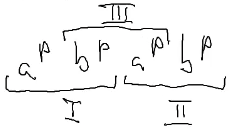
\includegraphics{./figures/string.png}
\end{figure}

Since $|vwx| \leq p$, the substring $vwx$ must be within one of the parts
$I, II, III$.
\begin{itemize}
        \item[part I] $vwx$ is inside the prefix $a^pb^p$ in the string
                $uv^2wx^2y$. The first symbol of the second half of
                the prefix is $b$ and the first symbol of the first half 
                is an $a$. Therefore, $uv^2wx^2y$ is not in $L_2$
        \item[part II] Similarly, if $vwx$ is inside the suffix $a^pb^p$
                in the string $uv^2wx^2y$ then the last symbol of the 
                first half is $a$ and the last symbol of the second half
                is $b$. Again, $uv^2wx^2y \not\in L_2$
        \item[part III] The last case is that $vxy$ is in the middle part.
                Now, $uv^0wx^0y = uwy$ is of the form $a^pb^ia^jb^p$
                where $i \neq p$ or $j \neq p$. Again, 
                $uv^0wx^0y \not\in L_2$, which produces \textbf{a 
                contradiction},
                and thus, $L_2$ is \textit{not} context free.
\end{itemize}
\end{document}

